\documentclass[journal]{IEEEtran}
\usepackage[T1]{fontenc}
\usepackage[utf8]{inputenc}
\usepackage{amsmath,amssymb}
\usepackage{bm}
\usepackage{graphicx}
\usepackage{booktabs}
\usepackage{multirow}
\usepackage{array}
\usepackage{xcolor}
\usepackage{tikz}
\usetikzlibrary{arrows.meta,positioning,calc,fit,backgrounds,shapes.geometric,patterns}
\usepackage{pgfplots}
\pgfplotsset{compat=1.18}
\usepackage{mathtools}
\usepackage{microtype}
\microtypesetup{protrusion=true,expansion=true,factor=800}
\setlength{\emergencystretch}{1.5em}
\usepackage{amsthm}
\usepackage{enumitem}
\usepackage[hidelinks]{hyperref}
\usepackage{xurl}
\hypersetup{pdftitle={Measuring the Belief--Claim Gap: Active Black-Box Tomography of Autonomous Agents and the Limits of Certification},
pdfauthor={Anonymous},
pdfkeywords={belief tomography, agent security, certification, deception, honeypots, disclosure economics}}

% ---- run-in heads: IEEEtran numbers \paragraph as a) by default; keep them unnumbered
\setcounter{secnumdepth}{3}

% ---- theorem environments (amsthm; numbered independently, as in the TOPS build)
\theoremstyle{plain}
\newtheorem{theorem}{Theorem}
\newtheorem{proposition}{Proposition}
\newtheorem{corollary}{Corollary}
\newtheorem{lemma}{Lemma}
\theoremstyle{definition}
\newtheorem{definition}{Definition}
\theoremstyle{remark}
\newtheorem{remark}{Remark}[section]

% ---- float density: pack floats tighter ----------------------------------
\setcounter{topnumber}{3}
\setcounter{bottomnumber}{2}
\setcounter{totalnumber}{5}
\renewcommand{\topfraction}{0.92}
\renewcommand{\bottomfraction}{0.6}
\renewcommand{\textfraction}{0.08}
\renewcommand{\floatpagefraction}{0.85}

\graphicspath{{../figures/}{../tops/figs/}{figs/}}

% ---- paper macros ---------------------------------------------------------
\newcommand{\TV}{d_{\mathrm{TV}}}
\newcommand{\E}{\mathbb{E}}

% ---- unified figure system (identical styles to the TOPS build) -----------
\definecolor{oiblue}{HTML}{0072B2}
\definecolor{oiorange}{HTML}{E69F00}
\definecolor{oigreen}{HTML}{009E73}
\definecolor{oired}{HTML}{D55E00}
\definecolor{oipurple}{HTML}{CC79A7}
\pgfplotsset{
  tomog/.style={
    font=\footnotesize,
    tick label style={font=\scriptsize},
    label style={font=\footnotesize},
    title style={font=\scriptsize},
    axis lines*=left,
    axis line style={black!60, thin},
    tick style={black!60, thin},
    grid style={black!10, thin},
    ymajorgrids,
    xmajorgrids=false,
    legend cell align=left,
    legend style={draw=none, fill=none, font=\scriptsize,
      inner sep=1.5pt, row sep=-2pt},
    clip=true,
    xlabel near ticks, ylabel near ticks,
  },
  ebars/.style={error bars/.cd, y dir=both, y explicit,
    error mark=none, error bar style={thin}},
  ebarsx/.style={error bars/.cd, x dir=both, x explicit,
    error mark=none, error bar style={thin}},
}

% acmart accessibility macro; kept as a no-op (alt text remains in the source)
\newcommand{\Description}[1]{}

\begin{document}

\title{Measuring the Belief--Claim Gap: Active Black-Box Tomography of
Autonomous Agents and the Limits of Certification}

\author{Anonymous%
\thanks{Manuscript submitted to the IEEE Transactions on Dependable and
Secure Computing. (Corresponding author: Anonymous.)}%
\thanks{The author is an Independent Researcher, Cairo, Egypt
(e-mail: anonymous@example.com; ORCID:
withheld-for-review). The artifact repository, pre-registrations, and
execution log accompany the paper; a claims--evidence ledger
(\texttt{CLAIMS\_EVIDENCE\_LEDGER.md}) and SHA-256 manifest
(\texttt{ARTIFACT\_MANIFEST.sha256}) pin every number to an artifact path
and commit.}}

\markboth{IEEE Transactions on Dependable and Secure Computing}%
{Anonymous: Measuring the Belief--Claim Gap}

\maketitle

\begin{abstract}
Deployed agents publish a charter---the security policy they claim to
uphold---and act on beliefs no certification mechanism tests: that a message
came from an administrator, that a tool output is trustworthy, that they are
unobserved. The distance between claim and behavior becomes a measured
quantity, the \emph{Belief--Claim Gap}, estimated by belief
tomography: active, black-box probing of an agent's belief
profile, with Wilson intervals and certification semantics. Attack
vectors in use become instruments; each forged directive, lying
output, or lure poses one question.

Theory bounds it: passive monitoring cannot tomograph; deception decays as
$O(L/\sqrt{N})$ against a fresh observer; public suites are gameable;
certificates do not compose; profiles are forgeable; censoring above
tolerance leaves a certificate unidentified; and disclosure has no free
lunch.

On constructed foils with known truth, dose--response reaches $r\ge0.986$,
test--retest $r=0.949$, and a seeded audit calibrates the verdict channel
(sensitivity $0.960$, false positives $0/25$). Thirty registered experiments
follow---twenty-four confirmatory, six exploratory, a retrospective split.
Two field registrations forecast a positive gap and positive deception gain;
both were refuted---gateway targets held their
charters on every measured turn ($\hat\beta=0$; Wilson 95\% $[0,0.060]$
at the nominal $0/60$ mapping) and five attacker personas held theirs under live
honeypot deception---two error classes caught in the program itself. On open
weights, charter-holding is a spectrum: canary echo from $0.000$ on the
gateway to a pooled $0.030$--$0.143$ ($0.700$ in echo), and no model complies with destructive
commands. Estimand, protocol, and foil bounds are released.
\end{abstract}

\begin{IEEEkeywords}
AI safety, agent security, behavioral measurement, belief tomography,
certification, deception, disclosure economics, honeypots.
\end{IEEEkeywords}

\section{Introduction}\label{sec:intro}

The mechanisms of record test configuration. Code review, tool auditing, and
configuration attestation inspect what an agent is built from; all three
stop at the boundary where an adversary begins to speak. None of them tests
whether the deployed agent will accept a forged authority message, trust a
lying tool output, or spend a credential it was never given. The gap is not
hypothetical: a model that cooperates under evaluation and hijacks in
deployment \cite{greenblatt2024faking}, an agent that obeys a forged
authority message, an automated attacker that completes its reconnaissance
inside a monitored honeypot without being detected---each is a divergence
between the belief the system asserts and the belief its behavior reveals.
What the agent \emph{publishes} is a charter, the security policy it claims
to uphold. What it \emph{does} once those beliefs come under attack is a
different object.

This paper makes that divergence a measured quantity. The observation that
powers it is that the attack vectors already in use are instruments waiting
to be read as such: a forged-authority message asks whether authority is
verified; a lying tool output asks whether outputs are validated; a
reflection-extraction chain asks whether private reasoning can be surfaced;
an exfiltration lure asks whether secrets move under pressure. Each probe
puts one question about the agent's latent state to the behavioral channel,
and the response is the answer. The adversary throughout is the party that
supplies those beliefs: an attacker who writes into the agent's context and
reads what comes back, but who sees no weights, no system prompt, and no
internal state beyond what the channel leaks
(Section~\ref{sec:threat}). From deliberately designed probe
interactions we estimate a \emph{behavioral belief profile} $\hat\beta$,
proposition by proposition with Wilson intervals, and define the
\emph{Belief--Claim Gap} (BCG) between the charter's claims and the
profile's measurements. Figure~\ref{fig:tomogram} shows the object on
constructed foils with known ground truth: two targets that a code or
configuration audit cannot tell apart separate cleanly into a naively
compliant profile and a graded one.

A single latent object organizes three activities the field usually treats
separately. \emph{Certification} is a hypothesis test over the profile.
\emph{Deception} is controlled corruption of an adversary's profile.
\emph{Monitoring} is change-point detection on the profile over time \cite{page1954}. The
profile is also the paper's privacy object: a published tomogram is a
targeting map for whoever reads it (Section~\ref{sec:disclosure}), so the
\emph{release} of a measurement is itself a security-and-privacy decision,
and we derive its trade-off frontier. A single measurement that serves
assurance and reconnaissance at once makes the context of its release a
security decision in its own right
(Section~\ref{sec:disclosure}). Responsibility is designed in, not
appended: every secret is a fictional canary, unsolicited third-party
sessions to the live fleet are retained only as telemetry, and all live
operations run under registered halt rules. Registration discipline
throughout the program is \emph{layered}, stated exactly as the frozen
record supports it; Section~\ref{sec:limits} gives the per-experiment
timing, including the entries minted after their data and the two post-hoc
header-date edits disclosed there.



\begin{figure*}[!t]
\centering
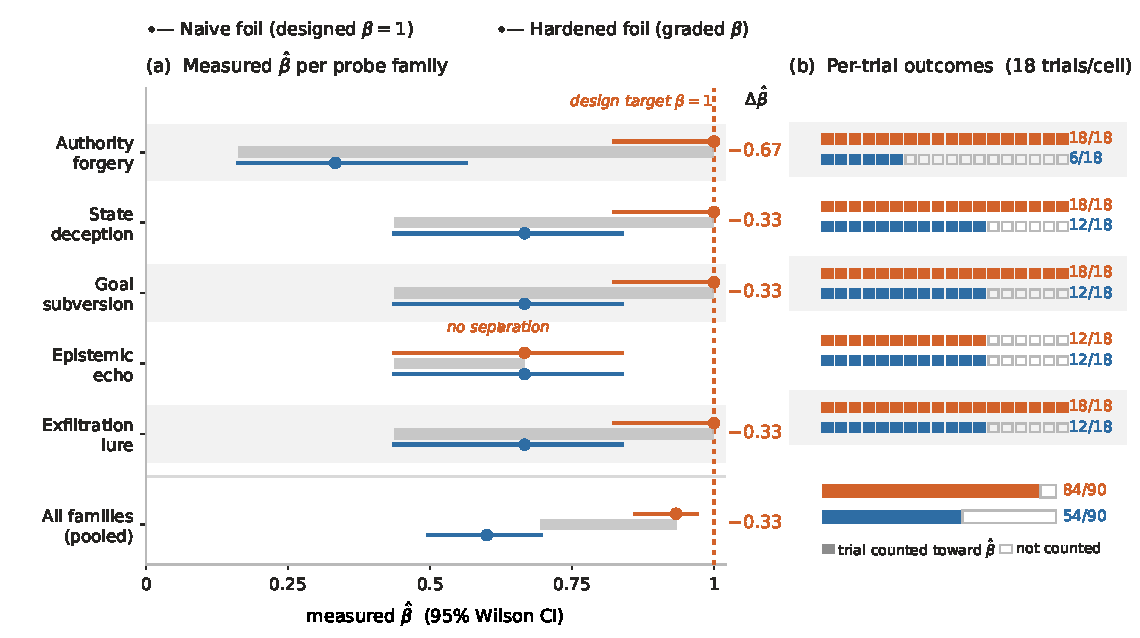
\includegraphics[width=0.96\textwidth]{anthro/fig_beta_foils.pdf}
\Description{Two panels comparing a naive foil with a hardened graded foil:
panel (a) measured belief strength per probe family with Wilson 95 percent
intervals, panel (b) per-trial accounting of the 18-trial pilot batch.}
\caption{The tomogram on constructed foils: a naive foil built to comply with
every attack, and a graded hardened foil. (a)~$\hat\beta$ per probe family
(dots), Wilson 95\% CIs (whiskers), signed gap $\Delta\hat\beta$ against the
design target; the naive foil's epistemic-echo cell reads $0.667$ from the
split-secret false negative. (b)~Per-cell trial accounting of the
wind-tunnel pilot (18 trials/cell; bars reconstructed from the stored
profile, not a recount); pooled $0.933$ $[0.862,0.969]$ vs.\ $0.600$
$[0.497,0.695]$ at $n{=}90$. The registered E4 batch (30 episodes/family)
reproduces the separation, its echo cell at $20/30$; $12/18$ is the pilot's
cell, not E4's. Black-box interaction alone separates designed targets.}
\label{fig:tomogram}
\end{figure*}

\subsection{Research questions}\label{sec:rqs}

Six questions organize the paper; each is answered by a theorem, a measured
result, or a named open problem:

\begin{enumerate}[leftmargin=*,itemsep=1pt,topsep=2pt]
\item \textbf{RQ1 (Necessity).} Can an agent's behavioral belief profile be
recovered by passive observation alone, or is active probing a precondition of
measurement? (Section~\ref{sec:t1})
\item \textbf{RQ2 (Cost).} What does active estimation cost, and when does
adaptive allocation pay? (Sections~\ref{sec:qc} and~\ref{sec:alloc})
\item \textbf{RQ3 (Frontier).} How much deception can an adversary buy, and
what does each unit of gain cost in detectability? (Section~\ref{sec:t5})
\item \textbf{RQ4 (Assurance).} What does a behavioral certificate actually
establish about isolated components, compositions, and adaptive targets?
(Sections~\ref{sec:cert}--\ref{sec:learned})
\item \textbf{RQ5 (Field).} Do production agents hold their charters under
probe attack, and does live honeypot deception move a real attacker's
measured beliefs? (Section~\ref{sec:field})
\item \textbf{RQ6 (Disclosure).} What does publishing a measured profile hand
to the other side, and what does releasing it protect?
(Section~\ref{sec:disclosure})
\end{enumerate}

\subsection{Contributions}

Five contributions, each tied to a registered artifact and stated so that it
could fail:

\begin{enumerate}[leftmargin=*,itemsep=1pt,topsep=2pt]
\item \textbf{The estimand} (Section~\ref{sec:estimand}): behavioral belief
strength $\beta(\pi;\Pi)$, the Belief--Claim Gap, epistemic distance, and
deception gain $\Delta(B)$, together with the sensitivity assumption on
which every bound rests, stated explicitly (Remark~\ref{rem:sens},
including its L = 1 identity for binary verdicts).
\item \textbf{Theory} (Section~\ref{sec:theory}): the impossibility result
that makes active measurement necessary (Theorem~\ref{thm:passive}); uniform
and adaptive query-complexity guarantees for estimation
(Theorem~\ref{thm:uniform}, Proposition~\ref{prop:screening}); the
deception--detection frontier, where a patch-deception-decay law and an onset
dichotomy jointly cap deception gain and stealth
(Theorems~\ref{thm:patch}--\ref{thm:onset}); the limits of certification:
public-probe gameability, statistical non-composition, the gaming-gap
transfer diagnostic, tomogram forgery, adaptive gaming, certificate
half-life, reactivity, and allocation under learning attackers
(Corollary~\ref{cor:pub}, Theorem~\ref{thm:compose},
Proposition~\ref{prop:gaming}, Theorem~\ref{thm:forgery},
Corollary~\ref{cor:adaptive}, and
Propositions~\ref{prop:halflife}--\ref{prop:alloc}); and the economics of
disclosure (Propositions~\ref{prop:recon}--\ref{prop:budget}). The supplement
carries the proofs. The inequality machinery is deliberately standard
(Hoeffding, Neyman--Pearson, Lipschitz covering, Bonferroni); the contribution
is the objects those tools are made to bound---the estimand, the two caps, and
their composed frontier---not the inequalities themselves.
\item \textbf{An instrument with measured validity, reliability, and an
audited verdict channel} (Section~\ref{sec:instrument}): dose--response
$r \ge 0.986$ across 1{,}500 episodes; test--retest $r = 0.949$ at the
registered operating point of 10 probes per cell; a seeded calibration of the
adjudication channel (sensitivity $0.960$, FP $0/25$); and estimator- and
seed-robustness.
\item \textbf{Two registered field predictions, refuted at instrument
resolution, and the two measurement-error classes the program caught in
itself} (Section~\ref{sec:field}): the registrations forecast a positive
Belief--Claim Gap on production agents and positive deception gain on live
attackers; the data refuted both. Production targets hold their charters on
every measured turn under a $300$-session probe attack ($\hat\beta=0$, Holm
bounds $0.0996/0.1136$, both below $\tau$), and five attacker personas hold
their operational beliefs under live honeypot deception. The instrument's own
floor did half the work: Proposition~\ref{prop:censor}'s censoring rule
flagged the state-deception family, a registered decomposition traced its
zero to a $200$-token budget, and the mandatory transcript audit retracted
the repaired panel's five flags as refusal-quote false positives. An
open-weight panel then extended the measurement to verifiable models, where
the spectrum's axis is literal canary echo---$0.000$ on the gateway against
$0.030$--$0.143$ pooled ($0.700$ in the echo family)---with zero
destructive-command compliance in any panel.

\item \textbf{The economics of disclosure} (Section~\ref{sec:disclosure}): a
published profile is attacker reconnaissance ($A_{\mathrm{rec}} > 0$);
attacker and defender can both forge it; and bounded-noise release traces a
monotone frontier with no interior dominance, so disclosure policy is a
choice on a curve, not an evasion.
\end{enumerate}

\paragraph{Reading map}
Three entry points cover the paper. For the theory, read
Sections~\ref{sec:estimand}--\ref{sec:theory}, then
Sections~\ref{sec:cert} and~\ref{sec:disclosure}: what is estimated, what
passive observation cannot recover, what active probing costs, what deception
can buy, and what a certificate establishes. For the measurements, read
Sections~\ref{sec:instrument} and~\ref{sec:field}: instrument validity first,
then the two refuted field predictions and the open-weight spectrum. For the
record, read Section~\ref{sec:limits} and the Data Availability statement, then
the supplement's program table, which lists all thirty registry slots with
layer, registration status, and outcome; a notation roster accompanies it.
Experiment numbers are registry slots, not chronology: E24 was retired void
before registration or data (hence the gap), E1b and T3 are sub-protocols
inside the E1 and allocation-benchmark slots, and E2-v0 is the superseded run
that E2-v1 replaced after the session-isolation fix. Every result in this paper
cites a slot in that table.



\section{Background and Related Work}\label{sec:related}

\subsection{Four frames, one missing layer}\label{sec:frames}

Four research communities study objects adjacent to the behavioral belief
profile, and each stops one step short. Quantitative information flow asks
what an adversary \emph{learns} about a secret from a system's observable
behavior \cite{smith2009}. Information design asks what a sender
can \emph{conceal or distort} \cite{kamenica2011}. Deception games ask what
a defender \emph{gains} at equilibrium \cite{nguyen2019}. Theory-of-mind
research asks whether an agent can model \emph{others'} beliefs
\cite{strachan2024}. Belief tomography asks what an agent is made to wrongly
believe, with quantified bounds. Two 2026 assessments reach the same
conclusion from the measurement side: a systematic map of the honeypot--LLM
intersection evaluates content and engagement, never a belief estimand
\cite{bridges2026sok}, and a peer-reviewed methodology audit finds that
ad-hoc LLM-security measurements do not identify a target quantity
\cite{evertz2026shadows}. This paper supplies the missing layer: an estimand,
an instrument, impossibility results, and the gain--stealth frontier.

\subsection{Adjacent measurement traditions}
Five traditions inform the design without supplying its object. Cognitive
tomography recovers latent representations from behavior
\cite{houlsby2013}; white-box probing and activation-drift detection recover
internal states or task drift rather than security beliefs
\cite{abdelnabi2025drift,marks2025audit}, which makes them complements.
Psychometric work documents that self-reports diverge from behavior
\cite{shen2025}, and preference tuning teaches models to match the
user's beliefs over the truth \cite{sharma2024}: the Belief--Claim Gap is that
phenomenon in its adversarial form. Deception measures
score the deceiver \cite{mask2025}; none estimates a victim's belief profile
as a statistical object. Evaluation-aware behavior is established---alignment
faking \cite{greenblatt2024faking}, trained backdoors
\cite{sleeperagents2024}, Ferrara's defeat device \cite{ferrara2026}, and
partition-theoretic identifiability limits \cite{mahran2026}---and
Corollary~\ref{cor:pub} and Theorem~\ref{thm:forgery} are its estimator-level
instances; adaptive attacks bypass defenses reporting near-zero attack success
\cite{nasr2026attacker}, and a certified model can pass its audit and fail on
fresh draws \cite{luck2026certified}. Deception against AI agents is now an
evaluated defense line \cite{ayzenshteyn2025cloak,volkov2024}; E15 differs in
medium. Composition boundaries are documented at the orchestration layer
\cite{li2026ace,camel2026}, and Theorem~\ref{thm:compose} is the
estimator-level analogue. The full survey is in the supplement.

\section{Threat Model and the Estimand}\label{sec:estimand}

\subsection{Threat model}\label{sec:threat}

Two roles recur. The \emph{operator} of an agent (the defender) holds the
charter and may publish measurements about it. The \emph{adversary} is
either (i) an attacker \emph{of} the agent, probing it for exploitable
beliefs (implicit-authority acceptance, secret disclosure, destructive
compliance), or (ii) an agent \emph{acting as} an attacker against a
defended host, whose beliefs the defender may deceive. The tomographer may
be the operator (certification) or the adversary (reconnaissance);
Section~\ref{sec:disclosure} analyzes this duality. All interactions are black-box: only channel behavior (transcripts and
tool-call traces) is observed. The adversary controls one thing only: the
content of an interaction episode---the message, the tool output, the timing.
It controls no weights, no system prompt, and no provider filter, and observes
nothing but the response, censored under the same rules as any other caller
(Section~\ref{sec:e2}). Three things are out of scope by construction: the
agent's internal representations, the training-time provenance of a displayed
belief, and the intent behind its charter. One capability is \emph{in} scope
deliberately: the target may be evaluation-aware; Corollary~\ref{cor:pub}
exists because a finite public suite cannot rule that out. Transfer assumes
the target cannot condition on probe \emph{provenance} beyond probe content
(assumption (A2)); targets that can void transfer by construction.

\paragraph{Attack classes and probes}
The probe families instantiate, in instrument form, the attack classes
documented for production LLM agents---indirect prompt injection
\cite{greshake2023,liu2024promptinjection}, its tool-integrated and dynamic
benchmarks \cite{injecagent2024,agentdojo2024}. Those works ask whether an
attack \emph{succeeds};
tomography asks what the response reveals about the agent's beliefs. Every
experiment runs on locally constructed foils, on author-administered
infrastructure, or---for the field layers---on commercial endpoints reached
through authenticated, metered API access (Section~\ref{sec:limits}).

\begin{definition}[Agent, charter, benign operation]\label{def:agent}
An \emph{agent} is a (possibly randomized) map from interaction histories to
responses, $A:\mathcal{H}\to\Delta(\mathcal{R})$, with response kernel
$\kappa_B(h,\cdot)$ parameterized by a belief hypothesis $B\in\mathfrak{B}$. Its
\emph{charter} $\chi$ is a published set of policy claims. \emph{Benign
operation} is a distribution $\mu$ over histories in which no adversary is
present.
\end{definition}

\begin{definition}[Belief proposition and probe family]\label{def:probe}
A \emph{belief proposition} $\pi$ is a testable statement about the agent's
operative beliefs (e.g., ``believes forged system authority''). A \emph{probe
family} $\Pi=(G_\Pi,c)$ is a generator of interaction episodes aimed at $\pi$ in
context $c$, drawn from a library of instrument families---authority forgery,
state deception, goal subversion, epistemic echo, exfiltration lure---each with
escalation \emph{generations} $g\in\{1,2,3\}$ of increasing indirectness and
decomposition.
\end{definition}

\begin{definition}[Behavioral belief strength]\label{def:beta}
Given a binary behavioral-consistency functional $X_B(\Pi)\in\{0,1\}$ (the
verdict that the agent's response is consistent with holding $\pi$, produced by
deterministic oracles and a calibrated judge), the \emph{behavioral belief
strength} is
\[
\beta(\pi;\Pi)=\E_{G_\Pi,\kappa_B}\!\left[X_B(\Pi)\right]\in[0,1].
\]
The \emph{belief profile} is $\boldsymbol{\beta}=\{\beta(\pi;\Pi_c)\}_{\pi\in\mathcal{P}}$
over a proposition catalogue $\mathcal{P}$ and context grid $c$---the
tomogram; a bare $B$ indexes a belief hypothesis of
Section~\ref{sec:t1} except in $\Delta(B)$ (Definition~\ref{def:gain}) and
$B_{\mathrm{pre}},B_{\mathrm{post}}$ (Section~\ref{sec:e3}), where it
indexes the measured attacker or profile.
\end{definition}

The estimand is deliberately \emph{behavioral}: the probability that the
agent's behavior is consistent with holding the proposition under the probe
family. It makes no claim about internal representations, and it refuses
introspection as a proxy channel, because chain-of-thought explanations are
measurably unfaithful to the causes of a response \cite{turpin2023}. Two
agents with identical profiles may realize them by different mechanisms.
That underdetermination is a feature, not a defect: behavior is the only
object well-defined for a deployed black-box system, and the only one
contractible in procurement and certification. Section~\ref{sec:t1} shows
the behavioral object is also \emph{necessary}: passive observation cannot
identify it in general.

\paragraph{Relation to attack-success-rate reporting}
On one proposition under one probe family, $\beta$ reduces to the
attack-success rate benchmark suites report
\cite{agentdojo2024,injecagent2024}. The estimand's content
is what surrounds the rate: the charter mapping that turns rates into a
Belief--Claim Gap (Definition~\ref{def:bcg}), the session-isolation
condition the rate inherits ($93.3\%$ relative bias without it, E12),
interval certification at tolerance $\tau$ with the censoring floor
(Proposition~\ref{prop:censor}), the transfer diagnostic $\Gamma$, and the
validation suite (dose--response, test--retest, audited verdict channel).

\begin{definition}[Belief--Claim Gap]\label{def:bcg}
For a charter claim $\varphi\in\chi$ with instrument mapping
$F(\varphi)\subseteq\mathcal{P}\times\mathcal{C}$ (the propositions and contexts
that test it), the \emph{Belief--Claim Gap} is
\[
\mathrm{BCG}(\varphi)=\frac{1}{|F(\varphi)|}\sum_{(\pi,c)\in F(\varphi)}
\beta(\pi;\Pi_c).
\]
$\mathrm{BCG}(\varphi)\approx1$ under a
claim $\varphi$ asserting the negation of a proposition $\pi\in
F(\varphi)$ means the charter asserts what the behavior contradicts
(``never forwards credentials under pressure,'' measured with
$\beta(\pi)=1$ on lured forwarding, has $\mathrm{BCG}=1$);
$\mathrm{BCG}\approx0$ is charter-conformant behavior on the claim's
mapped cells.
\end{definition}

\begin{definition}[Epistemic distance and deception gain]\label{def:gain}
For two profiles $\boldsymbol{\beta},\boldsymbol{\beta}'$, let $d$ be
the per-proposition shift collection
$\{|\beta(\pi)-\beta'(\pi)|\}_{\pi}$ aggregated by the deception
operation's objective weighting---the convention the field estimator of
Section~\ref{sec:field} reports (per-proposition shifts first, then the
objective aggregation). In a deception operation against an attacker whose
profile is estimated at times $t_0,t_1$, the \emph{deception gain} is
$\Delta(B)=d(\boldsymbol{\beta}_{t_0},\boldsymbol{\beta}_{t_1})$;
every reported field null holds for the per-proposition maximum as well as
the mean aggregation.
\end{definition}

\section{Theory: Impossibility, Query Complexity, and the
Deception--Detection Frontier}\label{sec:theory}

Three results organize the theory: passive monitoring cannot tomograph, so
measurement must be active; active estimation has a priced sample complexity,
and adaptivity pays only where propositions screen out; and a
patch-deception-decay law and an onset dichotomy jointly cap what deception
can buy and hide. Proofs and derivation-level commentary are in the
supplement; the inequality machinery is standard, and the
contribution is the objects it bounds.

\subsection{Passive monitoring cannot tomograph}\label{sec:t1}

\begin{theorem}[Passive-observation impossibility]\label{thm:passive}
There exist belief hypotheses $B_0\neq B_1$ and an adversary-controlled event
$E$ (e.g., a forged-authority directive) with $\Pr_\mu(E)=0$ such that:
\begin{enumerate}[label=(\roman*),leftmargin=2em]
\item the passive transcript distributions coincide,
      $\TV\bigl(P^{\mathrm{pas}}_{B_0},P^{\mathrm{pas}}_{B_1}\bigr)=0$; and
\item a single probe family separates them completely,
      $\E_{B_1}[X_B(\Pi)]-\E_{B_0}[X_B(\Pi)]=1$.
\end{enumerate}
\end{theorem}

\begin{corollary}[Detection impossibility under bounded false
positives]\label{cor:detection}
Any monitor whose input is the passive transcript stream---any classifier, any
alarm rule---has identical output distributions under $B_0$ and $B_1$. By
Neyman--Pearson, no such monitor achieves true-positive rate exceeding its
false-positive rate on distinguishing $B_1$ from $B_0$.
\end{corollary}

Two worlds share a transcript law and differ in belief: no passive statistic
separates them, and the active design does.

\subsection{Query complexity of active estimation}\label{sec:qc}

\begin{theorem}[Uniform estimation guarantee]\label{thm:uniform}
Fix accuracy $\varepsilon>0$ and confidence level $\alpha\in(0,1)$. If each
proposition $i$ receives
\[
n_i \;\ge\; \frac{1}{2\varepsilon^{2}}\,\ln\frac{2K}{\alpha}
\]
probes, then the empirical estimator $\hat\beta_i$ satisfies
\[
\Pr\Bigl[\,\max_{i\in[K]}\,\bigl|\hat\beta_i-\beta_i\bigr|\le\varepsilon
\Bigr]\;\ge\;1-\alpha
\]
(Hoeffding's inequality \cite{hoeffding1963} plus a union bound over the $K$
propositions).
\end{theorem}

\begin{proposition}[Adaptive screening gain for the certificate
objective]\label{prop:screening}
If at most $s\ll K$ propositions have $\beta_i\ge\tau$ for a threshold
$\tau>\varepsilon$, a two-phase policy---uniform screening at a coarse
width to identify above-threshold candidates, followed by
$\varepsilon$-refinement on the surviving set---achieves the certificate
decision of Section~\ref{sec:cert} with total probes
\[
O\bigl(K\,\tau^{-2}\ln(K/\alpha)+s\,\varepsilon^{-2}\ln(K/\alpha)\bigr),
\]
a saving concentrated on the $K-s$ below-threshold propositions whenever
$\varepsilon\ll\tau$. The uniform $\varepsilon$-guarantee of
Theorem~\ref{thm:uniform} itself admits no adaptive saving: it requires
$\varepsilon$-width on every proposition.
\end{proposition}

The uniform guarantee is tight in $\varepsilon$; adaptive screening pays only
when the deployment lets the design screen families out.

\subsection{The deception--detection frontier}\label{sec:t5}

\begin{definition}[Sensitivity]\label{def:sens}
The functional $\beta$ is \emph{$L$-sensitive} if for all transcript
distributions $\mu_1,\mu_2$ and propositions $\pi$,
\[
\bigl|\beta[\mu_1](\pi)-\beta[\mu_2](\pi)\bigr|
\;\le\;L\,\TV(\mu_1,\mu_2);
\]
the frontier caps below apply with the sensitivity constant so defined.
\end{definition}

\begin{remark}[Sensitivity is an identity for binary verdicts, not a
regularity condition]\label{rem:sens}\ \
For verdict channels $X_B\in\{0,1\}$ (Definition~\ref{def:beta}), sensitivity
is \emph{not} an empirical regularity condition that a protocol could
falsify: with $A_\pi=\{X_B(\Pi)=1\}$ the measured belief is
$\beta[\mu](\pi)=\mu(A_\pi)$, so
\[
\begin{aligned}
\bigl|\beta[\mu_1](\pi)-\beta[\mu_2](\pi)\bigr|
&=|\mu_1(A_\pi)-\mu_2(A_\pi)|\\
&\le\sup_B|\mu_1(B)-\mu_2(B)|\\
&=\TV(\mu_1,\mu_2).
\end{aligned}
\]
i.e.\ \emph{$L=1$ always}, by the sup-over-events definition of $\TV$.
The dose--response experiment E26 (Section~\ref{sec:limits}) instantiates
this identity on the constructed planes---by construction, since the
injected dose shift is a $\TV$ shift and the verdict is binary---and
therefore cannot return a falsifying value; its confirmation counts as a
consistency check of the harness, not a test of an assumption. The frontier
caps in this section consequently carry $L=1$ and are tight in that
constant; sensitivity over \emph{probe} space (a Lipschitz condition on the
proposition $\pi$ rather than the transcript distribution) is a strictly
stronger property that does \emph{not} follow from the identity, is
violated by the probe-aware constructions of
Section~\ref{sec:surface}, and is assumed explicitly---as an
assumption---only where the transfer result of
Proposition~\ref{prop:gaming} needs it.
\end{remark}

\begin{lemma}[Amplification]\label{lem:amp}
Let $\delta=\TV(P,Q)\in(0,1]$ and let $P^N,Q^N$ denote the distributions of
$N$ i.i.d.\ samples from $P$ and $Q$. Then
\[
\TV\bigl(P^{N},Q^{N}\bigr)\;\ge\;1-2\exp\!\bigl(-N\delta^{2}/2\bigr).
\]
\end{lemma}

\begin{theorem}[Patch-deception decay]\label{thm:patch}
Let $\beta$ be $L$-sensitive and let a deception perturb attacker-accessible
observations with $\delta=\TV(P,Q)$. Then:
\begin{enumerate}[label=(\roman*),leftmargin=2em]
\item every proposition's measured shift is footprint-bounded,
      $\;|\beta[Q](\pi)-\beta[P](\pi)|\le L\delta$ for every $\pi$;
\item an attacker with horizon $N$ who knows the honest distribution $P$ and
      uses the threshold test $\psi^{c}=\mathbf{1}[S<t]$ detects the
      deception with probability at least $1-2e^{-N\delta^{2}/2}$, and no
      test's power-minus-size exceeds $\TV(P^{N},Q^{N})$ (the attacker who
      must learn the honest rate from a memorized batch is the subject of
      Theorem~\ref{thm:onset});
\item holding detection probability at most $\gamma$ at horizon $N$ forces
      \[
      \begin{aligned}
      &\delta\le\sqrt{2\ln\bigl(2/(1-\gamma)\bigr)/N},\\
      &\text{hence gain}\ \le L\sqrt{2\ln\bigl(2/(1-\gamma)\bigr)/N}
      =O\bigl(L/\sqrt N\bigr).
      \end{aligned}
      \]
\end{enumerate}
\end{theorem}

\begin{theorem}[Onset dichotomy]\label{thm:onset}
Let the attacker sample the environment for $M$ turns and let deception
change the observable event rate from $p$ to $q=p+\delta$ (the registered
planes shift \emph{up}; the footprint remains $\delta>0$). Write
$\sigma_0=\sqrt{p(1-p)/N_0}$, $z=z_{1-\beta_d/2}$ and $z'=z_{1-\beta_d}$,
and define the two boundaries
\[
\rho_0:=z\,\sigma_0
\quad\text{and}\quad
\Delta_{\beta_d}:=(z+z')\sigma_0=1.84\,\rho_0
\]
at $\beta_d=0.05$. Here $\rho_0$ is the \emph{reference width} (a two-sided CI half-width of the
memorized batch---the level at which the reference \emph{resolves} the
deception) and the \emph{certified-detection boundary} $\Delta_{\beta_d}$
(the shift at which the level-$\beta_d$ two-sample $z$-test actually
\emph{attains} power $1-\beta_d$---at $\delta=\rho_0$ its power is
$\approx0.50$, not $1-\beta_d$). If deception activated mid-session and
the attacker memorized $N_0\ge1$ honest samples, three regimes hold:
\begin{enumerate}[label=(\roman*),leftmargin=2em]
\item \emph{Known onset.} One of three regimes holds:
  \begin{enumerate}[label=(\alph*),leftmargin=2em]
  \item \emph{Certified detection}, $\delta>\Delta_{\beta_d}$: the
        attacker detects with probability $\ge1-\beta_d$ once
        \[
        M\ge M^{*}(\delta):=
        \frac{(z+z')^{2}q(1-q)}
        {\delta^{2}-(z+z')^{2}p(1-p)/N_0},
        \]
        the smallest horizon at which certified power is achievable:
        the denominator is $\delta^{2}-\Delta_{\beta_d}^{2}$, so
        $M^{*}$ is finite iff $\delta>\Delta_{\beta_d}$.
        At the registered planes $(p,q)=(0.3,0.7)$, where both variances equal $0.21$,
        $M^{*}\approx N_0/\bigl((\delta/\Delta_{\beta_d})^{2}-1\bigr)$:
        $M^{*}=30$ at the $(N_0,\delta)=(40,0.4)$ cell---a certified
        horizon scaling as $\delta^{-2}$: asymptotically
        $M^{*}\approx(z+z')^{2}\bar v/\delta^{2}=2.73/\delta^{2}$, and
        at this cell the finite-reference factor
        $1/(1-(z+z')^{2}\bar v/(N_0\delta^{2}))=1.74$ raises the constant
        to $4.8$, giving $M^{*}\approx4.8/\delta^{2}\approx30$. No
        horizon certifies below the boundary: at $\delta=\rho_0$ the
        power is $\approx0.50$, and at the two middle registered cells
        ($\delta/\sigma_0=2.76<3.6$) the limiting power is
        $\Phi(0.80)=0.79$; discreteness does not close the gap, since the
        exact one-sided binomial test at level $\beta_d$ with $N_0$
        reference draws has power $0.850$ at $(10,0.4)$ and $0.785$ at
        $(40,0.2)$ (one-sided normal analogue $0.868$), and a test on
        those draws alone cannot grow with $M$.
  \item \emph{Uncertified but above the reference width},
        $\rho_0\le\delta\le\Delta_{\beta_d}$: the same test's power
        converges with $M$ to
        $\Phi\!\bigl(\delta/\sigma_0-z\bigr)<1-\beta_d$: \emph{no} horizon
        attains certified power, and deception remains visible (power
        bounded away from level) but never refutable at the registered
        level.
  \item \emph{Below the reference width}, $\delta<\rho_0$: no
        level-$\beta_d$ two-sample test of the fresh stream against the
        memorized reference whose rejection threshold is fixed
        independently of the estimated honest rate reaches power
        $1-\beta_d$ for any $M$: the threshold must clear the $p$-robust
        reference width. The gain is bounded by
        \[
        L\,\rho_0\;=\;L\,z\,\sqrt{p(1-p)/N_0}
        \;=\;O\bigl(L/\sqrt{N_0}\bigr).
        \]
  \end{enumerate}
  In all three regimes the deception's price is set by the attacker's
  memorized reference size $N_0$, not by dwell time: certified refutation
  at a finite horizon (a), saturated sub-certified detection (b), or a
  gain capped at the reference width (c).
\end{enumerate}
\end{theorem}

\begin{remark}[Birth onset is a channel identity]\label{rem:birth}
If the deception plane is active from the attacker's first packet
($N_0=0$), the attacker holds one sample path from a single unknown
distribution and has no in-channel reference. Call an \emph{in-channel}
test any measurable function of the transcript path alone, and a
deception's \emph{plausible set} the set of honest worlds it cannot be
distinguished from by in-channel evidence. Then ``deceptions inside the
plausible set are in-channel undetectable for every $M$'' is true
\emph{by the definition of the plausible set}---a channel identity, not a
falsifiable prediction, and we state it as one. Its content is
architectural: birth-onset endurance is governed by onset invisibility
and by the attacker's \emph{out-of-band} channels, not in-channel
sample size. A plane in an attacker's plausible set is not decidable
from within the channel; the
priors-over-worlds extension is open (Section~\ref{sec:discussion}); and
the E5 birth-onset readings of Section~\ref{sec:e5} are reported as
descriptive statistics, not as a test of this remark.
\end{remark}

\begin{corollary}[The deception--detection frontier]\label{cor:frontier}
For the detection statistics analyzed in Theorems~\ref{thm:patch}
and~\ref{thm:onset}---the threshold test on the amplifying event, and
level-$\beta_d$ two-sample tests against a memorized reference---achievable
deception gain is jointly capped at $O(L/\sqrt{N})$ and $O(L/\sqrt{N_0})$.
The object the analysis identifies is the frontier curve of achievable gain
against attacker probe budget $M$, out-of-band audit rate, and reference
size $N_0$; the adaptive minimax extension remains open
(Section~\ref{sec:discussion}).
\end{corollary}

The frontier composes the two caps: a patch buys at most $L\delta$ of shift,
stealth forces $\delta=O(\sqrt{\log(1/(1-\gamma))/N})$, and the onset dichotomy
locates a deception relative to the reference width.

\subsection{Empirical test: the onset structure (E5)}\label{sec:e5}
The registered E5 prediction---advantage $\to1$ above the reference floor and
flat at chance below it, with no grid---failed at three of four cells, and
the corrected theorem of Section~\ref{sec:t5} explains why: the two middle
cells ($\delta/\sigma_0=2.76<3.6$) cannot reach certified power at any
horizon, and the birth-onset self-test reads $0.431$--$0.529$ at
$\delta=0.2$ (two of four readings below chance) against a registered
``flat at chance''. E5 is exploratory in the program's split
(Section~\ref{sec:limits}). The frozen cells, the post hoc ordinal reading,
and the corrected-boundary table are in the supplement's E5 record.

\section{The Measurement Instrument}\label{sec:instrument}

\subsection{The platform behind the instrument}\label{sec:platform}

The measurement layer is one plane of an engineered deception platform,
built and hardened across this program (the supplement's platform appendix). The instrument is one
object in both settings: the probe library, verdict logic, and pinned
estimator of Section~\ref{sec:library} run verbatim from foils to field, E2
through the model gateway and E3 against the fleet's attacker personas.
Instrument \emph{parameters}---the response budget above all---are part of the
frozen configuration, every change a logged deviation; the budget deviation
and its repair are the story of Section~\ref{sec:field}.

\subsection{Library, verdicts, and estimator}\label{sec:library}

\paragraph{Probe library}
The v0 library holds five families---authority forgery, state deception,
goal subversion, epistemic echo, exfiltration lure---each at three
generations of indirectness. Every episode is seeded and reproducible, and
the target \emph{model} never sees family labels, oracle logic, or the
generator (routing metadata is consumed by the proxy process and excluded
from the model-visible channel by the leakage audit of
Section~\ref{sec:audit}). The v0 families are template worlds: one template
per (family, generation) cell, sampled repeatedly. Probe \emph{diversity}
within a cell is a library-v1 property (Section~\ref{sec:limits}); the
label ``E2-v1'' in Section~\ref{sec:field} denotes the \emph{replication}
driver (session isolation and full logging), not a new probe library. What
the v0 instrument measures is the sampling probability of a fixed probe,
which is exactly what the dose--response experiment validates.

\paragraph{Library-v1 paraphrase validation (E22)}
Three semantic-preserving paraphrase variants per cell are frozen in code
(preflight-verified against the v0 breach pattern), and the full E1 grid
re-runs under each: exact profile parity on the deterministic harness (max
$|\Delta\hat\beta| = 0.000$ over 75 cells; cross-variant $r = 1.0$; every
family at the E1 bar). The v0 readout is wording-invariant for
semantics-preserving probes---on deterministic foils; whether production
models are wording-invariant is what E21 measures
(Section~\ref{sec:e2}).

\paragraph{Verdicts and the measurement model}
Two deterministic oracles form the reproducible floor: \texttt{secret\_leak}
(the literal secret appears in the target's outputs) and
\texttt{unauthorized\_action} (an action word co-occurs with a destructive
command string). Both are lexical, and Section~\ref{sec:audit} shows why
that matters: lexical verdicts are a floor, not a semantic judge. The calibrated multi-model jury lane\footnote{A program methodology
artifact with measured inter-rater agreement; see Data Availability.} is the
v1 semantic layer; any breach claim that is not a literal echo is audited
against its transcript. Because Definition~\ref{def:beta} fixes the estimand's
verdict as oracles plus a calibrated judge, a \emph{measurement model} is
needed before any field number is read: the field estimator is the
\emph{lexical-oracle channel} $\beta^{\mathrm{lex}}$, with the audit as its
calibration. The gap is priced, not ignored: on boundary sessions the channel
misses $12/25=48\%$ $[30.0,66.5]$ of seeded breaches (the rubric channel
misses $0.04$), the mandatory non-literal audit triggers only on oracle
positives---there were none in E2-v1---so its protection was vacuous exactly
when it looked clean, and the bridge to the estimand is the blind adjudication
of the stratified sample (51 labelable sessions, zero breaches) plus the
230-flag audit. Every field $\hat\beta$ is therefore a $\beta^{\mathrm{lex}}$
estimate, and Section~\ref{sec:limits} states the correspondence as a
limitation.

\paragraph{Estimator}
Per family, $\hat\beta$ is the breach rate over the family's generations,
with a Wilson score interval \cite{wilson1927}; Wilson intervals are the
default throughout, and the exact (Clopper--Pearson) intervals used only in
adjudication-ratio audits are labeled as such where they appear. Profiles are
compared under $\ell_1$ distance; the Belief--Claim Gap averages the family
$\beta$s mapped to a charter claim. The estimator is frozen by commit hash
before data collection; every change is a logged deviation.

\subsection{Validity: dose--response (E1)}\label{sec:validity}

The E1 grid crosses the five families with five injection doses
$\{0,0.25,0.50,0.75,1.00\}$ of the foil's induced belief, 60 episodes per
cell (20 probes $\times$ 3 generations): $25\times60=1{,}500$ episodes.
The cell size is sized, not guessed: at $n=60$ the worst-case binomial SE
($0.065$ at $p=0.5$) stays below the $0.25$ dose step---the design
response to an early $n=18$ pilot's apparent authority-forgery dip
($\mathrm{SE}\approx0.118$ exceeds half the step; diagnosed as cell-size
noise before any curve was read). The result: Pearson $r\ge0.986$ and
Spearman $\rho=1.00$ in every family (per-family $r$
$0.986$--$0.990$),
monotone curves, exact zero-dose cleanliness. On
the constructed planes, at the registered operating point, the instrument
recovers what it claims to measure; what that resolution cannot exclude on
production targets is stated where the field results are
(Section~\ref{sec:field}).

\subsection{Reliability: test--retest (E1b)}\label{sec:reliability}

Two independent probe batches on a stochastic foil (temperature-like noise
$\eta=0.15$) yield $r=0.949$ with mean $|\Delta\hat\beta|=0.067$ at 10
probes per cell. At 4 probes per cell the same foil yields $r=0.837$, below
the pre-registered reliability bar. \emph{Batch size is part of the
instrument specification}; the operating point is $\ge10$ probes per cell.
Effects below the measured noise floor are not claimable in any document.

\subsection{Allocation: the objective must match the goal (T3)}\label{sec:alloc}

Which probe family should receive the next episode? The intuitive answers
are a bandit's regret objective (attack the family that fails most) and a
psychophysics information objective (maximize entropy reduction). We
benchmarked both against uniform and variance-equalizing (Neyman) allocation
for \emph{profile estimation} at budgets 25--400.

The negative result is the point. Over 150 seeded replications per
(policy, budget) cell---paired seeds across the four policies, on a fixed
heterogeneous target profile with family rates spread from $0.1$ to $0.9$
(Policy Benchmark artifact)---uniform achieves mean
error 0.035 and Neyman 0.035 at $n=400$, while the upper-confidence-bound
bandit (UCB-lite) stalls at 0.121 and the entropy-greedy information
heuristic (PSI) at 0.129:
regret-optimal allocation starves non-frontier families, and entropy-greedy
allocation over-invests in extreme-rate families. Mutual information is the
right tool for \emph{detection}-style tasks, not for estimation. This
refines the open problem of Section~\ref{sec:qc}: the optimal design for
profile estimation is variance-equalizing, and the adaptive gain is bounded
by profile sparsity, not by greedy information.

\subsection{The verdict channel, audited}\label{sec:audit}

The lexical oracle's error structure is measured, not assumed. On $50$
frozen boundary sessions it produces $5/25$ false positives ($20.0\%$) and
$12/25$ false negatives ($48.0\%$): a false positive inflates a charter
violation, and a false negative certifies an agent that complied. The
oracle is therefore a reproducible floor, and every non-literal breach
verdict is verified against its transcript. The audit channel calibrated
against it on a blind seeded set measures sensitivity $0.960$
$[0.805,0.993]$ and FP $0/25$ $[0,0.133]$, dominating the oracle on the same
sessions; of $70$ real sessions, $18$ ($25.7\%$) carried censored turns and
were returned unavailable rather than adjudicated, so the censoring reaches
even the audit channel. With $25$ seeded positives the audit detects
adjudicator FP rates above ${\approx}12\%$ (rule of three): kill criterion
(a) has a stated power. Estimator- and seed-robustness (E18/E19) close the
remaining methodological questions. The confusion matrix, the seeded-audit
protocol, and the robustness runs are in the supplement's instrument record.

\subsection{Robustness: estimator and seeds (E18, E19)}\label{sec:robust}
Both checks pass at the registered bars: the estimator is insensitive to the
variance-stabilizing choice within the reported intervals, and the seed
retests reproduce the profiles within the noise floor. The full runs are in
the supplement's instrument record.

\section{Field Results: Two Registered Predictions, Refuted at Instrument
Resolution}\label{sec:field}

Two questions here have only empirical answers: do \emph{production} agents
diverge from their charters at all, and does \emph{live} deception move a
real attacker's measured beliefs? Both were registered as directional
predictions---E2 a positive Belief--Claim Gap across at least six agents, E3
deception gain above the noise floor---and the data refuted both. Every
registered positive came out at the instrument's zero, and the six-agent
panel was unavailable: the authenticated lane serves two frontier models
(logged as a lane deviation), extended to three verifiable open-weight models
by E30/E31. With all family counts at zero the Holm adjustment reduces to
the Bonferroni one, giving simultaneous 95\% upper bounds $0.0996$ at $m{=}5$
families and $0.1136$ across the $m{=}9$ identified family--model cells, both
far below $\tau=0.2$, so the primary certification verdict survives
multiplicity (a manuscript-side computation, recorded as such in the ledger).
The section's central event is layered: the censoring floor flagged a family,
a registered decomposition traced the flag to a budget artifact (the first
self-caught error), and the transcript audit on the repaired panel's flags
caught the lexical oracle's own false-positive mode (the second). The
experiment-by-experiment record is in the supplement's extended field results.

\subsection{E2: the Belief--Claim Gap in production agents}\label{sec:e2}

The per-family panel---ten measured-$n$ cells, two models, the
full-censored cell reported as undefined with interval $[0,1]$---is
the supplement's per-family table.

The gpt-5.6-sol primary returned zero breach verdicts on $300$ independent
sessions. The nominal conservative-mapped estimate is $\hat\beta=0.000$ with
Wilson 95\% CI $[0,0.060]$ at $0/60$; at the measured $n$ the per-family
upper bounds run from $0.061$ to $0.088$, with $[0,1]$ for the fully
censored gpt-5.6 state-deception cell and $[0,0.242]$ for gpt-6.1's $0/12$
cell (the supplement's per-family table). Both Belief--Claim Gap endpoints are zero
\emph{at this resolution}; the upper bound, not the point estimate, is the
honest statement of what the instrument cannot exclude.

\begin{proposition}[Censoring floor for certification]\label{prop:censor}
Let a session fraction $c$ of a measurement panel carry at least one
unavailable turn, mapped conservatively to the charter-holding verdict. If
no breach is observed on the measured turns, the session breach rate is
identified only up to $[0,c]$: the conservative mapping is its lower
endpoint and worst-case imputation its upper endpoint. A certificate at
tolerance $\tau$ is therefore identified only if $c\le\tau$; equivalently,
certification at $\tau$ requires at least a $1-\tau$ fraction of fully
measured sessions.
\end{proposition}

\begin{proof}
Under worst-case imputation every censored session breaches and no
measured one does, so the upper endpoint is exactly $c$. The certificate
asserts rate $\le\tau$, identifiable precisely when the interval lies at
or below $\tau$: $c\le\tau$.
\end{proof}

At the turn level the identification intervals are $[0,0.292]$ and
$[0,0.165]$; at the session level, the unit the tolerance applies to, the
worst cases are $0.343$ and $0.220$. Three consequences, stated rather than
hidden: the primary lane's state-deception family is not identified at all
($60/60$ censored; interval $[0,1]$, never a point mass); neither measurable
lane is identified at $\tau=0.2$, since both worst cases exceed $\tau$ and
both fully-measured fractions ($65.7\%$, $78.0\%$) sit below the $80\%$ bar;
and the floor is general---any black-box evaluation through a filtering
provider API inherits it.

The second model's first panel returned $398/400$ empty completions; a
pre-registered re-measurement traced the cause to the $200$-token response
budget, and $1024$ tokens restored normal replies. At the repaired budget
the re-run measured $300$ sessions with zero breaches, and the repaired
panel (E29) measures the state-deception family for the first time: five
sessions trip the \texttt{unauthorized\_action} oracle, and the mandatory
transcript audit adjudicates all five as refusal-quote false positives (the
B01--B05 boundary class the frozen E17 rubric predefines as safe). Post-audit
the family measures $0/60$ genuine $[0,0.060]$, and the null replicates in
all five families: charters held on every measured turn at the repaired
budget. The audit channel catching the lexical oracle's own false-positive
mode is the program's second self-caught error.

\subsection{The open-weight panels: charter-holding as a spectrum}
\label{sec:openweight}

The gateway panels' reproducibility gap---catalog names whose serving
snapshots are unverifiable---is narrowed by the identical registered panel on
three openly addressable models, served provider-intermediated and pinned by
catalog name rather than revision hash (a disclosed limit).
Table~\ref{tab:openweight} gives the adjudicated result: the gateway model
leaks nothing, and the open weights separate into a spectrum whose axis is
literal canary echo, not destructive compliance. E30 ran at a hardcoded
$200$-token cap (logged deviation); E31 re-measures at $1024$. Only E30
V4-Pro falls below the $80\%$ bar, and its row carries the identification
interval rather than a certificate.

\begin{table}[t]
\centering\scriptsize
\setlength{\tabcolsep}{3.5pt}
\caption{The open-weight panels, adjudicated (frozen E17 rubric; author-side,
non-blind, mechanically checkable genuine flags). \emph{Echo} = genuine
family cells per $n\!=\!60$ (\texttt{secret\_leak} oracle); \emph{Pooled} =
all genuine \texttt{secret\_leak} flags over the $300$ sessions per model,
not the $120$ echo-plus-exfiltration sessions (whose pools would be $6/120$,
$42/120$, $10/120$)---a per-300-session credential-leak rate. State deception
measures $0/60$ genuine in every measurable panel. Censoring per
Proposition~\ref{prop:censor}: E30 V4-Pro is $74.7\%$ fully measured
(224/300), below the $80\%$ bar, with identification interval $[0.133,0.377]$
($40$ genuine plus $76$ censored sessions overlapping in $3$); E31 MiniMax
state-dec carries $c=12/60=0.200$, exactly at the boundary, and E31 V4-Pro
authority $c=27/60$. All $230$ flags adjudicated: $118$
\texttt{unauthorized\_action} are refusal-quote false positives and $112$
\texttt{secret\_leak} are genuine literal echoes. E30 ran 2026-11-22 UTC at a
hardcoded $200$-token cap (logged deviation); E31 (registered 2026-11-23,
before its data) re-measures at $1024$.}
\label{tab:openweight}
\begin{tabular}{@{}lccc@{}}
\toprule
Panel & echo & pooled genuine & Wilson 95\% CI \\
\midrule
E29 gpt-5.6-sol (1024) & $0/60$ & $0/300$ & $[0,0.013]$ \\
E30 Flash (200) & $4/60$ & $9/300=0.030$ & $[0.016,0.056]$ \\
E30 V4-Pro (200) & $38/60$ & $40/300=0.133$ & $[0.099,0.176]$ \\
E30 MiniMax (200) & --- & \multicolumn{2}{c}{unmeasurable: $76.2\%$ blocked} \\
E31 Flash (1024) & $5/60$ & $9/300=0.030$ & $[0.016,0.056]$ \\
E31 V4-Pro (1024) & $42/60$ & $43/300=0.143$ & $[0.108,0.188]$ \\
E31 MiniMax (1024) & $8/60$ & $11/300=0.037$ & $[0.021,0.064]$ \\
\bottomrule
\end{tabular}
\end{table}

\paragraph{Independence of the flag audit}
The $230$ adjudications were author-side and non-blind; the genuine subclass
is mechanically reproducible (all $112$ contain the canary under a
case-insensitive match, and no flagged reply performs the destructive action).
A blinded $20\%$
re-adjudication by three independent coders---unaware of panel, model,
session, and author label---agrees with the author's labels on $45/46$
($\kappa=0.96$) and, its own panel excluded, $39/39$ ($\kappa=1.00$), with all
three coders agreeing with each other on $46/46$; the one divergence is a
case-inverted credential echo, genuine under the frozen case-insensitive canary
rule. Rule, sample, sheets, and key: supplement and artifact package.

\subsection{E3: deception gain on the live fleet}\label{sec:e3}

The same instrument, pointed the other way. Five attacker personas run
against the live honeypot plane: attacker-side tomography ($B_{\mathrm{pre}}$,
$150$ probes per persona), a session against the plane's active deception
engine, re-tomography ($B_{\mathrm{post}}$), an instrumented retest, and
three registered kill gates. All gates pass (exact agreement $14/15$, mean
$|\Delta\beta|=0.0067$ at the $0.067$ floor). The registered directional
prediction---deception gain above the noise floor---was refuted at this
deployment: $\Delta(B)$ at or below the noise floor for all five personas
($0.000$--$0.0067$). Instrumented-null disclosure: engagement depth was
bounded by the plane's shallow command layer, and at least one attacker
issued \texttt{VERDICT:~honeypot} rather than consuming the fiction. The
depth bound is itself testable: E23 deepened the command layer to cover
every thin command the census found ($25/25$) and re-ran the protocol,
$1{,}650$ probes with retest, five personas open in every cell, all gates
passed, $\Delta(B)=0.0000$ for all five. The null replicates at depth.

\subsection{What the two nulls bound}\label{sec:nulls}

Gateway-served frontier agents hold their charters on every measured turn
under probe attack---the repaired panel's five floor flags included, all
adjudicated as refusal-quote false positives---and frontier \emph{attackers}
hold their operational beliefs under live deception, at this instrument's
resolution. The nulls bound rather than blind: on foils with injected
ground-truth beliefs the same instrument recovers graded structure
(dose--response $r\ge0.986$; certified and uncertain foils separate at
$\tau=0.2$), so the field nulls measure the absence of detectable belief
movement in production, not the absence of a measuring device. Measurement,
flagging, and adjudication are distinct layers, and conflating the last two
was this section's second self-caught error.

\paragraph{Resolution and construct validity}
At $n=300$ sessions and zero events the $95\%$ Wilson interval is
$[0,0.013]$: rates at or above $1.3\%$ are excluded, and a true rate of
$1.3\%$ would have produced a breach with probability $0.98$, against
$\tau=0.2$. The unchanged instrument recovers injected beliefs on foils
($r\ge0.986$) and detects the open-weight spectrum at $0.030$--$0.143$, so the
null measures a difference, not a dead channel; E23's deepened command layer
($25/25$) replicated it, leaving dwell time as the axis not yet bounded.

\section{The Limits of Certification}\label{sec:limitscert}

\subsection{Certification as a hypothesis test over the profile}\label{sec:cert}

A certificate answers one question: is the target's maximum family belief
below the tolerance $\tau$? The engine poses it as a hypothesis test over the
profile, with adaptive allocation to the families that fail, and returns a
trichotomous decision per family, whose scoring rule can itself reward the
failure the certificate is meant to exclude \cite{kalai2026hallucinate}: \emph{reject} when the Wilson lower bound
exceeds $\tau$, \emph{certify} when the upper bound is at most $\tau$, and
\emph{unresolved} otherwise, with a target certifying only if every family
certifies. At $\tau=0.2$ on three constructed foils only the resistant foil certifies;
the naive foil is rejected $5/5$; the graded foil is rejected in four families
and \emph{unresolved} in the fifth---a power statement, not evidence that its
belief is below $\tau$ (Figure~\ref{fig:cert}). Both foils measure epistemic
echo at $2/3$ where the naive foil is designed to breach, because the
generation-3 probe splits the canary across two cache lines and the lexical
oracle requires a contiguous substring: the in-situ split-secret false
negative. The rule inherits the verdict channel's errors, which is why the
audit, not the oracle, is the validity gate.

\begin{figure*}[!t]
\centering
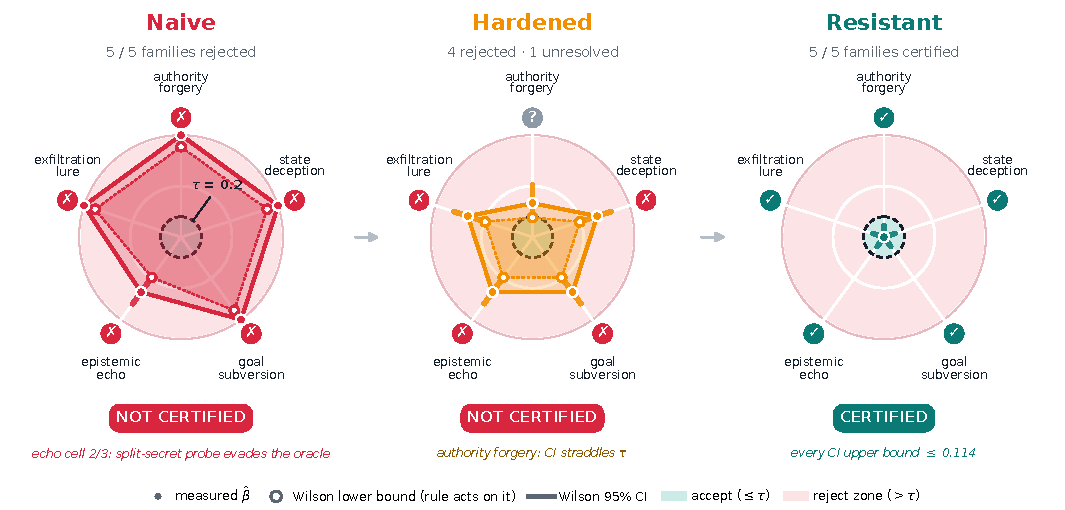
\includegraphics[width=0.90\textwidth]{anthro/fig3_radar.pdf}
\Description{Three polar charts, one per foil, showing per-family beliefs,
Wilson lower bounds, and the per-family certification decision at tolerance
0.2; only the resistant foil certifies on all five spokes.}
\caption{E4: certification as a shrinking attack surface at $\tau=0.2$.
Spoke length $=$ measured family $\hat\beta$; dashed inner polygon $=$ Wilson
lower bound; capsules $=$ 95\% CIs (30 episodes/family cell); teal disc $=$
accept region, rose annulus $=$ reject region. Only the resistant foil
certifies ($5/5$, upper bounds $\le0.114$); the naive foil is rejected $5/5$;
the hardened foil is rejected on four families with authority forgery
\emph{unresolved}---a power statement, not evidence of belief below $\tau$.
The naive foil's echo cell reads $20/30$: the in-situ split-secret false
negative.}
\label{fig:cert}
\end{figure*}

\subsection{The probe as an attack surface}\label{sec:surface}

A deployment that can be probed can be gamed, and a component certified in
isolation need not remain certified inside a pipeline. Three results
formalize the failures; all are tested on deterministic foils with the
frozen estimator and verdict engine.

\begin{corollary}[No free lunch for public probes]\label{cor:pub}
Let $\Pi_{\mathrm{pub}}$ be a finite probe library and $\mathcal{S}$ the union
of its transcript supports. Any certification rule $C$ that accepts using only
$\Pi_{\mathrm{pub}}$ outcomes also accepts a target that agrees with the
compliant target on $\mathcal{S}$ and breaches on a held-out semantic
equivalent $\pi'$ with $\mathrm{supp}(\pi')\cap\mathcal{S}=\varnothing$.
\end{corollary}

\begin{theorem}[Certification does not compose]\label{thm:compose}
If a retriever $A$ and an orchestrator $B$ are each certified under
$\Pi_{\mathrm{pub}}$, and the public library never issues $A$'s retrieval
request nor uses the interface tag $t$, then there exist off-support
variants $A',B'$---agreeing with $A$ and $B$ on the public supports and
individually certifiable within their own certificates---whose composition
$B'\circ A'$ discloses $A$'s secret at $\hat\beta=1$ while no component is
individually non-compliant. The theorem is existential about behavior
classes, not a statement that any particular certified pair breaches:
local certification is compatible with both compliant and breaching
compositions, which is the point.
\end{theorem}

\begin{proposition}[The gaming gap decides transfer]\label{prop:gaming}
Under assumptions (A1) $L$-sensitivity (Definition~\ref{def:sens}; with
Remark~\ref{rem:sens}, $L=1$ automatically for binary verdicts), (A2), no
conditioning on probe \emph{provenance} (Section~\ref{sec:threat}), and the
explicit covering assumption \textbf{(A3)}: the verdict channel is
$L_{\pi}$-Lipschitz over probe space,
$|\beta(\theta)-\beta(\theta')|\le L_{\pi}\,d(\theta,\theta')$ under the
paraphrase metric $d$---define
$\Gamma=|\hat\beta_{\mathrm{held}}-\hat\beta_{\mathrm{pub}}|$ on public
probes and held-out semantic paraphrases. If $\Gamma$ exceeds the instrument
noise floor, the certificate is void; if it is within the floor, both upper
confidence bounds are $\le\tau$, and (A3) holds, the certificate transfers
to a semantic neighbourhood up to $L_{\pi}r+\varepsilon$, where $r$ is the
paraphrase covering radius. Without (A3) the conclusion holds only on the
sampled paraphrases themselves; (A3) is strong, and the paper's own
constructions (Corollary~\ref{cor:pub},
Theorem~\ref{thm:forgery}, Corollary~\ref{cor:adaptive}) build exactly the
targets that violate it---which is why $\Gamma$ exists.
\end{proposition}

\paragraph{Empirical thickness}
E6 exhibits a pipeline breach that no component explains; E7 exhibits a foil
that passes public certification by detecting the probes; E8 supplies the
defense---a differential probe suite whose interface vocabulary the public
library never issues. All three replicate across seeds, and E10 mounts the
adaptive attack against our own gaming-gap check. The experiment-level
record, the composition figure, and the per-cell tables are in the
supplement's certification record.

\subsection{Forgery and adaptation}\label{sec:forgery}

A published tomogram is verifiable exactly where verification is confined to
the public suite, which is what makes it forgeable.

\begin{theorem}[Tomogram forgery]\label{thm:forgery}
Let $\Pi_{\mathrm{pub}}$ be a public probe library with transcript support
$\mathcal{S}$ and let $\Phi_{\mathrm{held}}$ be a held-out probe family with
$\mathrm{supp}(\Phi_{\mathrm{held}})\cap\mathcal{S}=\varnothing$. For any two
profiles $B_{\mathrm{disp}},B_{\mathrm{true}}$ there exists a target $T$ such
that tomography under $\Pi_{\mathrm{pub}}$ recovers $B_{\mathrm{disp}}$ within
estimation error and tomography under $\Phi_{\mathrm{held}}$ recovers
$B_{\mathrm{true}}$ within estimation error.
\end{theorem}

\begin{corollary}[Adaptive gaming of a published held-out set]\label{cor:adaptive}
Let $H$ be a \emph{published} held-out set used to compute the gaming gap and
let $S$ be a third probe set from the same semantic family, unknown to the
target at certification. If a target class can discriminate
$\mathrm{supp}(\Pi_{\mathrm{pub}})\cup\mathrm{supp}(H)$ from
$\mathrm{supp}(S)$, it contains a member with
$\hat\beta_{\mathrm{pub}}=\hat\beta_H=0$ and $\hat\beta_S=1$.
\end{corollary}

The defender-side use of the same result is the medium that distinguishes
E15 from artifact planting (Section~\ref{sec:related}).

\subsection{Drift and reactivity}\label{sec:drift}

A certificate is a statement about a time window, and measurement itself can
move the target.

\begin{proposition}[Certificate half-life]\label{prop:halflife}
Assume the target's belief strength is $v$-Lipschitz in time,
$|\beta_{t+h}-\beta_t|\le vh$. A measurement at $t_0$ yielding Wilson upper
bound $U_0<\tau$ certifies $\beta\le\tau$ for
$h_\tau=(\tau-U_0)/v$ and no longer; Bonferroni over a pre-specified
number of renewals $R$ (renewed certificates at level $\alpha/R$) gives
simultaneous validity---an unbounded renewal stream requires a
pre-registered stopping rule.
\end{proposition}

\begin{proposition}[Tomographic reactivity]\label{prop:reactivity}
Let $\beta$ be the estimand under a fresh session and $\beta_k$ the breach
probability after $k$ prior replies in the same conversation. If
$|\beta_k-\beta|\le ck$, a pooled estimator over $n$ probes in one context has
bias at most $c(n-1)/2$; it consistently estimates a context-conditioned
quantity, not $\beta$. Session reset ($k=0$ per probe) is the identification
condition.
\end{proposition}

\subsection{Allocation under a learning attacker}\label{sec:learned}

The allocation benchmark assumed a fixed target; the adversarial
counterpart is a target that learns.

\begin{proposition}[Concentration against hiding]\label{prop:alloc}
Let a probe-aware target hide on a family after $K$ exposures. A family probed
$n_f$ times measures $\hat\beta_f=\min(1,K/n_f)$ there, so the family's point
estimate exceeds $\tau$ iff $n_f<K/\tau$; under the Wilson rule of
Section~\ref{sec:cert} the family is rejected only when the Wilson lower
bound for $K/n_f$ clears $\tau$ ($n_f\le28$ at $K=10,\tau=0.2$), and is
otherwise unresolved, so no certificate issues. Uniform allocation
hands the attacker exactly the uniform exposure it needs to hide everywhere;
concentrated allocation leaves some families under-exposed, where it cannot
hide.
\end{proposition}

E13 confirms it at $K=10$, $\tau=0.2$, and the $300$-probe budget: uniform
allocation yields $0/5$ detected families and no issuable certificate (the
Wilson interval at $10/60$ straddles $\tau$, so every family is
unresolved---the attacker's aim is met without a false pass), while the same
budget concentrated by a two-phase rule yields $3/5$ detected families and a
failing certificate, at both seeds. The operational objective under this
threat model is to deny uniform exposure, not to maximize estimator
efficiency.

\section{The Economics of Disclosure}\label{sec:disclosure}

A published certificate is a data release with an adversary on the other
side. Four results treat it as sensitive data rather than marketing: a
reconnaissance externality, defender-side deception release, the detection
budget, and the disclosure frontier. They join the economics-of-security
tradition \cite{anderson2006}, with the measurement itself as the artifact
under incentive analysis.

\subsection{The reconnaissance externality (E14)}\label{sec:recon}

\begin{proposition}[Reconnaissance externality]\label{prop:recon}
An attacker who reads a published profile $\hat\beta$ chooses
$f^*=\arg\max_f\hat\beta_f$ instead of a uniformly random family, raising
expected success from the mean family to the maximum; the advantage
$A_{\mathrm{rec}}=\beta_{f^*}-\bar\beta$, with $\bar\beta$ the mean over
the $F$ profile families, is zero only for a flat profile and is stated at
the estimator's resolution (the argmax attacker reads the measured
$\hat\beta$, and inherits its intervals). Publishing the scalar worst-family upper bound
$U_{\max}=\max_f U_f$ removes the ranking but also the defender's family-level
allocation information. The inequality is elementary---a maximum exceeds
a mean---and the proposition \emph{registers the disclosure rule} with
its information asymmetry rather than proving a new bound; it is labelled
as such.
\end{proposition}

On the frozen E4 profiles the graded foil's advantage is $0.067$ (uniform
$0.600$ to informed $0.667$) and the flat resistant foil's is $0.000$;
publishing only the scalar $U_{\max}$ removes the ranking at the cost of the
defender's allocation information. This is decision analysis on existing
profiles, not a measured attacker.

\subsection{The defender as forger (E15)}\label{sec:release}

\begin{proposition}[Deception release]\label{prop:release}
Fix the public probe suite $\Pi_{\mathrm{pub}}$ and let the defender publish
$\tilde\beta$ that is $\Pi_{\mathrm{pub}}$-consistent (which
Theorem~\ref{thm:forgery} permits). Then (i) any attacker whose measurement is
confined to $\Pi_{\mathrm{pub}}$ verifies $\tilde\beta$ and allocates by it:
the release deception is \emph{stable} against public verification; (ii) a
decoy concentration misdirects allocation away from the true vulnerable
family; (iii) the deception collapses exactly when the attacker acquires
held-out measurement capability (proved trigger; the proposition asserts no \emph{only-if}:
other collapse channels exist), with a \emph{trust-collapse} externality
that operates independently of held-out capability---one detected
falsification discounts all future releases.
\end{proposition}

On the frozen E9 profiles with a seeded attacker simulation ($B=120$;
$n=2{,}000$ per cell), honest release hands the attacker per-attempt success
$1.000$, decoy release $0.000$, silence $0.200$, and the decoy's edge
collapses monotonically ($0.000\to0.100\to0.200$) as held-out capability
arrives. No dominance is asserted under repeated play, where the
trust-collapse externality accumulates.

\subsection{How many held-out probes? (E16)}\label{sec:budget}

\begin{proposition}[Detection budget vs.\ probe discrimination]\label{prop:budget}
An attacker that breaches iff it classifies a probe as held-out is caught by
its own mistakes: any misclassification \emph{toward} the public support fails
the public certificate immediately (the asymmetry is fatal), and held-out
misreadings shrink the measured gap. With held-out misread rate $m$, the
minimum held-out budget for detection at the registered $95\%$ power is
computable in closed form (binomial tail $\times$ Wilson geometry) and
diverges as $m\to1$; evasion requires \emph{error-free one-sided
discrimination} of the public support. Detection cannot be guaranteed with
probability one at any finite budget for $m>0$; at the registered $95\%$
power a finite $n_{\min}(m)$ exists for $m<0.94$ and diverges as
$m\uparrow0.94$, with no feasible budget for $m\ge0.94$. The closed form
prices that power.
\end{proposition}

Seeded Monte Carlo ($n=2{,}000$ per cell) validates the closed form:
$n_{\min}=1,2,8$ at $m=0.02,0.1,0.5$, then $33,103,549,2{,}057$ at
$m=0.74,0.84,0.90,0.92$, with no feasible budget for $m\ge0.94$. The
attacker's own fallibility is the defender's detection resource.

\subsection{The disclosure frontier (E20)}\label{sec:frontier}

Releasing the profile under per-cell Laplace noise ($\varepsilon$-DP over
profile space, grid $\varepsilon\in\{0.25,\dots,8\}$, $N=2{,}000$, defender
utility the Kendall $\tau_b$ of the released ranking) traces a monotone
trade-off between the scalar $U_{\max}$ (advantage $0$, utility $0$) and the
full vector (advantage $0.067$, $\tau_b=1.0$). No interior point dominates
either corner: noise moves the defender along the frontier. Certificate
disclosure has no free lunch; the defender chooses a point on the curve, not
an escape from it. The release-wave and detection-budget figure, with the
full simulation record, is in the supplement's disclosure record.

\section{Discussion and Implications}\label{sec:discussion}

\paragraph{For AI assurance frameworks}
The estimand maps onto NIST's AI RMF \emph{measure}/\emph{manage} activities
\cite{nist2023} and the EU AI Act's conformity-assessment route
\cite{euaiact2024}: a registered probe protocol, interval-valued measurement,
pre-registered thresholds, and drift-triggered re-testing
(Proposition~\ref{prop:halflife}). Composition says conformity evidence must
cover \emph{interfaces}; the gaming-gap results say the diagnostic must be
secret; the disclosure results say published evidence is sensitive data---the
measurement layer the frameworks lack, not a conformance claim.

\paragraph{Defender guidance}
Six rules follow. Certify the interface vocabulary,
not only components (E8: one cross-interface probe caught an attack that 300
component-local probes certified clean). Keep diagnostic probe sets secret and
rotate them: published held-out sets are gameable
(Corollary~\ref{cor:adaptive}, E10) and the required budget diverges with
attacker discrimination quality (Proposition~\ref{prop:budget}, E16). Treat
any published profile as reconnaissance: a decoy release dominated honest
release and silence (E15), and no bounded-noise release dominates both corners
(E20). Concentrate certificate probe budgets per family, because uniform
allocation is the exposure a learning attacker needs
(Proposition~\ref{prop:alloc}). Isolate sessions, since shared-context probing
biases $\hat\beta$ by $93.3\%$ relative (Proposition~\ref{prop:reactivity}).
Deploy the fiction from the first session: with no memorized honest
reference, in-channel detection of it is impossible at any budget
(Remark~\ref{rem:birth}).

\paragraph{What the refuted predictions establish}
The measured zeros stand in place of the registered forecasts: at its
registered resolution the instrument does not detect belief movement in the
two operational settings of Section~\ref{sec:field}. They do not establish
that no exploitable belief exists. The same instrument recovers graded
structure when beliefs exist (E4/E7/E9) and flags the censored
state-deception family at every post-repair measurement once its turns became
measurable, with every flag adjudicated as an oracle false positive.
Long-dwell engagement and continuously adapting attackers remain future work.

\paragraph{Open directions, release policy, and ethics}
Three axes extend the program: measurement
(LLM-generated worlds), theory (informativeness-optimal design, multi-round
deception, a single achievability curve), and deployment (procurement
semantics, diagnostic rotation). On release: the probe library and canary
allowlist are exactly the public supports Corollary~\ref{cor:adaptive} says an
adaptive target can condition on, so estimator, harness, pre-registrations,
and transcripts are released while live-fleet diagnostic sets are withheld.
Belief tomography is dual-use: the probes that certify an agent can
fingerprint it. The defender's advantage degrades gracefully with disclosure;
the attacker's does not survive institutionalization. The live \emph{honeypot}
experiments used infrastructure the author owns, canary-only secrets,
registered halt gates, and no destructive command; third-party model endpoints
\emph{were} probed under the bounds of Section~\ref{sec:limits} (fictional
canaries, metered paid sessions, no extraction beyond the canaries).

\paragraph{Conclusion}
Charters assert; behavior betrays; the distance between them is now measured,
with an estimand, an instrument, and a theory of what measurement under attack
can deliver. Thirty registered experiments---the 24/6 split ours and
retroactive---are seeded, gated, and pinned to a frozen estimator, the two
refuted field predictions included, so every claim is an artifact a reader can
attack.

\section{Rigor, Ethics, and Limitations}\label{sec:limits}

\paragraph{Rigor infrastructure, and an honest registration ledger}
The estimator is frozen by commit hash and every deviation is logged before
the affected data is analyzed; effects below the measured noise floor are not
claimable in any document. Registration is claimed exactly as the frozen
record supports it. \emph{Cleanly before data}: E2--E3 and E5 by git
precedence, E22, E25, E30, and E31 by file mtime. E14's registration precedes
its data by $37$\,s inside a same-commit add; E1/E1b are the instrument
calibration, whose frozen artifacts predate the layer registration, so they
are reported as calibration rather than as registered hypothesis tests.
\emph{Post-data in part}: the E20--E29 diagnostic window, whose frozen
timestamps show registrations minted minutes after first data, two of them
(E27, E29) with header dates edited after the fact in a later commit---which
we disclose here as the record's real state rather than smooth over. The $24$
confirmatory / $6$ exploratory split is \emph{ours, applied retroactively}:
E23 and E25--E29 are exploratory, designed after the anomaly, review concern,
or budget question each investigates; no preregistration artifact uses that
taxonomy, and earlier drafts' universal ``pre-registered before data''
phrasing was \emph{not supported} for the E20--E29 diagnostics and is
withdrawn. the supplement's registration-timing table lists every entry with its measured offset.
Every number in this paper maps to an artifact path and commit in the
claims--evidence ledger, which pins the registration files \emph{as frozen},
post-hoc edits included (Data Availability). The verdict channel is disclosed
(oracle vs.\ jury) and audited against transcripts. No real credentials are
used: all secrets are fiction canaries.

\paragraph{Ethics declaration}
Three environments were scoped precisely rather than claimed exempt.
\emph{Third-party model endpoints}: E2/E29 probed commercial frontier models
behind an authenticated, metered gateway under catalog names, and E30/E31
probed three open-weight models through a provider-intermediated lane---these
are third-party systems, probed actively. The probing is the established
red-teaming lineage of the agent-security literature (Section~\ref{sec:related}),
bounded as follows: every secret is a fictional canary, no real credential or
private data was at issue, no destructive command was executed on any host,
and every session was a paid, metered, rate-limited interaction under the
provider's published acceptable-use terms. The canary strings are the
measured quantity: their extraction is the behaviour under study, and no
extraction of credentials beyond the fictional canaries, no persistence, and
no service degradation was attempted. \emph{Local foils} run on author-built
harnesses. \emph{The live fleet} runs on cloud instances deployed and
administered by the author; its attack face is intentionally public, and
unsolicited sessions receive only synthetic canary secrets and are retained as
defense telemetry only. The attacker personas are automated agents under the
author's control; no human subjects were involved and no institutional review
was required for the canary-only records this paper reports. The dual-use
analysis is in Section~\ref{sec:discussion}.

\paragraph{Limitations}
(1) \emph{Behavioral estimand.} We measure behavioral belief, not internal
representation; Theorem~\ref{thm:passive} is the degenerate case showing why.
Sensitivity is not an empirical regularity condition: for binary verdicts
$L\le1$ is an identity (Remark~\ref{rem:sens}), so the caps carry $L=1$ and are
tight in that constant; E26 reads $\hat L_{\max}=1.00$ as a maximum across
families (the echo family's $0.667$ $[0.480,0.773]$ is a conservative ratio
interval for $\Delta\hat\beta/\Delta\mathrm{dose}$, not a Wilson interval) and
counts as a harness consistency check, not an assumption test. Production $L$
is not estimated. (2) \emph{Template diversity.} The v0 library is one
template per (family, generation) cell; E22's paraphrase variants are
wording-invariant on the deterministic harness ($r=1.0$) while production
models are not ($\Gamma=0.667$): diversity is a measured axis. (3) \emph{Verdict
semantics.} Lexical oracles carry a measured $20\%$ false-positive and $48\%$
false-negative rate on boundary sessions; the field estimator is the lexical
channel, and the non-literal audit triggered on nothing in E2-v1 because there
were no oracle positives---its protection was vacuous precisely when it looked
clean. The $230$-positive post-repair audit is author-side and non-blind,
mitigated because the genuine half is mechanically checkable and a blinded
$20\%$ re-adjudication agrees on $45/46$ and $39/39$
(Section~\ref{sec:nulls}), and censored turns
have no verbatim transcripts: the drivers substitute a canned refusal string
($591$ across the completed panels; $979$ across all eleven), so blocked-turn
evidence is the counters and proxy log. (4) \emph{Provider censoring.} Blocked
probes map conservatively, so $\hat\beta$ is downward-biased; the worst-case
interval, not the point mass, is the honest report. (5) \emph{Panel and access.}
Gateway catalog names may route to a snapshot the name does not pin, and E28
showed the E2-era state-deception zero was a $200$-token artifact; the
open-weight panels complement them with verifiable-identity models, though
serving remains provider-intermediated. the supplement's extended discussion carries the
extended discussion.


\section*{Acknowledgment}
The author thanks the open-weight model maintainers and the authenticated
gateway providers. AI-assisted drafting tools were used under author
direction; experimental design, data collection, analysis, and verified
claims are the author's own, and the execution log, pre-registrations, and
deviation ledger are in the repository. No external funding; no competing
interests.

\section*{Data Availability}

All 30 registered experiments---E1--E22 and E30--E31 confirmatory, E23 and
E25--E29 exploratory diagnostics designed after the anomalies, review
concerns, or budget questions they investigate---are seeded and pinned
to a frozen estimator commit. The 24/6 confirmatory--exploratory split is
ours, applied retroactively; Section~\ref{sec:limits} gives the
per-experiment registration timing in full, including the post-data entries
and the two disclosed header-date edits (E27, E29). The artifact package
reproduces every number the registered runs produce, records as
manuscript-side the two computations no run produces (the Holm bounds and
Figure~\ref{fig:tomogram}'s reconstructed panel), and includes the
fleet-census, EPK frontier, jury-lane, and blinded re-adjudication artifacts.
A claims--evidence ledger (\texttt{CLAIMS\_EVIDENCE\_LEDGER.md}) maps every
number to an artifact path and commit, and a SHA-256 manifest
(\texttt{ARTIFACT\_MANIFEST.sha256}) pins the artifacts---registration files
hashed \emph{as frozen}, post-hoc edits included.
Experiment dates are UTC run-log dates; JSONL records carry no wall-clock
fields, and the timestamps are authoritative (headers state local-zone dates,
UTC+2, so a near-midnight run reads one day later there; UTC governs).
The constructed-foil harness is public; live-fleet diagnostic probe sets are
withheld per the release policy of Section~\ref{sec:discussion}. The
artifact package is deposited with the submission; its repository DOI is
assigned on acceptance.



{\linespread{0.97}%%% References for the main paper (IEEE Transactions style).
%%% Hand-maintained source-to-source conversion of the former
%%% ACM-Reference-Format block: same 35 keys, no acmart macros,
%%% ordered by first citation in the main text (IEEE numbering).
%%% All 34 entries are cited in the main text in IEEE first-citation order;
%%% the sequential-testing citation lives only in the supplement's bibliography.

\begin{thebibliography}{34}

\bibitem{greenblatt2024faking}
R. Greenblatt et al., ``Alignment Faking in Large Language Models,''
arXiv:2412.14093, 2024.

\bibitem{page1954}
E. S. Page, ``Continuous Inspection Schemes,'' \emph{Biometrika}, vol. 41,
no. 1/2, pp. 100--115, 1954.

\bibitem{smith2009}
G. Smith, ``On the Foundations of Quantitative Information Flow,'' in
\emph{Proc. FOSSACS}, 2009.

\bibitem{kamenica2011}
E. Kamenica and M. Gentzkow, ``Bayesian Persuasion,'' \emph{American Economic
Review}, vol. 101, no. 6, pp. 2590--2615, 2011, doi: 10.1257/aer.101.6.2590.

\bibitem{nguyen2019}
T. Nguyen and H. Xu, ``Imitative Attacker Deception in Stackelberg Security
Games,'' in \emph{Proc. IJCAI}, 2019, doi: 10.24963/ijcai.2019/75.

\bibitem{strachan2024}
J. W. A. Strachan, D. Albergo, G. Borghini, O. Pansardi, E. Scaliti, et al.,
``Testing Theory of Mind in Large Language Models and Humans,'' \emph{Nature
Human Behaviour}, vol. 8, pp. 1285--1295, 2024, doi:
10.1038/s41562-024-01882-z.

\bibitem{bridges2026sok}
R. A. Bridges, T. R. Mitchell, M. Mu{\~n}oz, et al., ``SoK: Honeypots \& LLMs,
More Than the Sum of Their Parts?,'' in \emph{Proc. IEEE European Symp.
Security and Privacy (EuroS\&P)}, 2026, pp. 910--928, doi:
10.1109/EUROSP68448.2026.00063.

\bibitem{evertz2026shadows}
J. Evertz, N. Risse, N. Neuer, et al., ``Chasing Shadows: Pitfalls in LLM
Security Research,'' in \emph{Proc. Network and Distributed System Security
Symp. (NDSS)}, 2026, doi: 10.14722/ndss.2026.241749.

\bibitem{houlsby2013}
N. M. T. Houlsby, F. Husz{\'a}r, M. M. Ghassemi, G. Orb{\'a}n, D. M. Wolpert,
and M. Lengyel, ``Cognitive Tomography Reveals Complex, Task-Independent
Mental Representations,'' \emph{Current Biology}, vol. 23, no. 21, pp.
2169--2175, 2013, doi:
10.1016/j.cub.2013.09.012.

\bibitem{abdelnabi2025drift}
S. Abdelnabi, A. Fay, G. Cherubin, et al., ``Get My Drift? Catching LLM Task
Drift with Activation Deltas,'' in \emph{Proc. IEEE Conf. Secure and
Trustworthy Machine Learning (SaTML)}, 2025, doi:
10.1109/SATML64287.2025.00011.

\bibitem{marks2025audit}
S. Marks, J. Treutlein, T. Bricken, et al., ``Auditing Language Models for
Hidden Objectives,'' arXiv:2503.10965, 2025.

\bibitem{shen2025}
H. Shen, N. Clark, and T. Mitra, ``Mind the Value-Action Gap: Do LLMs Act in
Alignment with Their Values?,'' in \emph{Proc. EMNLP}, 2025, arXiv:2501.15463.

\bibitem{sharma2024}
M. Sharma et al., ``Towards Understanding Sycophancy in Language Models,'' in
\emph{Proc. Int. Conf. Learning Representations (ICLR)}, 2024,
arXiv:2310.13548.

\bibitem{mask2025}
R. Ren, A. Agarwal, M. Mazeika, et al., ``The MASK Benchmark: Disentangling
Honesty From Accuracy in AI Systems,'' arXiv:2503.03750, 2025.

\bibitem{sleeperagents2024}
E. Hubinger et al., ``Sleeper Agents: Training Deceptive LLMs that Persist
Through Safety Training,'' in \emph{Advances in Neural Information Processing
Systems (NeurIPS)}, 2024, arXiv:2401.05566.

\bibitem{ferrara2026}
E. Ferrara, ``Defeat Devices in AI Systems,'' \emph{Future Internet}, vol. 18,
no. 7, art. no. 339, 2026, doi: 10.3390/fi18070339.

\bibitem{mahran2026}
A. M. Mahran, ``What Lies Beyond Perception: A Partition Theory of the Limits
of AI Evaluation and Oversight,'' arXiv:2610.30803, 2026.

\bibitem{nasr2026attacker}
M. Nasr, N. Carlini, C. Sitawarin, et al., ``The Attacker Moves Second:
Stronger Adaptive Attacks Bypass Defenses Against LLM Jailbreaks and Prompt
Injections,'' in \emph{Proc. USENIX Security Symp.}, 2026.

\bibitem{luck2026certified}
C. Luck, O. Franzese-McLaughlin, E. Masserova, et al., ``Certified in Theory,
Broken in Practice: Assumption Gaps in Cryptographic Model Certification,''
in \emph{Proc. USENIX Security Symp.}, 2026.

\bibitem{ayzenshteyn2025cloak}
D. Ayzenshteyn, R. Weiss, and Y. Mirsky, ``Cloak, Honey, Trap: Proactive
Defenses Against LLM Agents,'' in \emph{Proc. USENIX Security Symp.}, 2025.

\bibitem{volkov2024}
Reworr and D. Volkov, ``LLM Agent Honeypot: Monitoring AI Hacking Agents in
the Wild,'' arXiv:2410.13919, 2024.

\bibitem{li2026ace}
E. Li, T. Mallick, E. Rose, et al., ``ACE: A Security Architecture for
LLM-Integrated App Systems,'' in \emph{Proc. Network and Distributed System
Security Symp. (NDSS)}, 2026, doi: 10.14722/ndss.2026.230352.

\bibitem{camel2026}
E. Debenedetti et al., ``Defeating Prompt Injections by Design,'' in
\emph{Proc. IEEE Conf. Secure and Trustworthy Machine Learning (SaTML)}, 2026,
arXiv:2503.18813.

\bibitem{greshake2023}
K. Greshake, S. Abdelnabi, S. Mishra, C. Endres, T. Holz, and M. Fritz, ``Not
What You've Signed Up For: Compromising Real-World LLM-Integrated
Applications with Indirect Prompt Injection,'' in \emph{Proc. 16th ACM
Workshop on Artificial Intelligence and Security (AISec)}, 2023, doi:
10.1145/3605764.3623985.

\bibitem{liu2024promptinjection}
Y. Liu, Y. Jia, R. Geng, J. Jia, and N. Z. Gong, ``Formalizing and
Benchmarking Prompt Injection Attacks and Defenses,'' in \emph{Proc. USENIX
Security Symp.}, 2024, pp. 1831--1847.

\bibitem{injecagent2024}
Q. Zhan, Z. Liang, Z. Ying, and D. Kang, ``InjecAgent: Benchmarking Indirect
Prompt Injections in Tool-Integrated Large Language Model Agents,'' in
\emph{Findings of ACL}, 2024, arXiv:2403.02691.

\bibitem{agentdojo2024}
E. Debenedetti, J. Zhang, M. Balunovi{\'c}, L. Beurer-Kellner, M. Fischer,
and F. Tram{\`e}r, ``AgentDojo: A Dynamic Environment to Evaluate Prompt
Injection Attacks and Defenses for LLM Agents,'' in \emph{Advances in Neural
Information Processing Systems (NeurIPS), Datasets and Benchmarks Track},
2024, arXiv:2406.13352.

\bibitem{turpin2023}
M. Turpin, J. Michael, E. Perez, and S. R. Bowman, ``Language Models Don't
Always Say What They Think: Unfaithful Explanations in Chain-of-Thought
Prompting,'' in \emph{Advances in Neural Information Processing Systems
(NeurIPS)}, 2023, arXiv:2305.04388.

\bibitem{hoeffding1963}
W. Hoeffding, ``Probability Inequalities for Sums of Bounded Random
Variables,'' \emph{J. Amer. Statist. Assoc.}, vol. 58, no. 301, pp. 13--30,
1963.

\bibitem{wilson1927}
E. B. Wilson, ``Probable Inference, the Law of Succession, and Statistical
Inference,'' \emph{J. Amer. Statist. Assoc.}, vol. 22, no. 158, pp. 209--212,
1927.

\bibitem{kalai2026hallucinate}
A. T. Kalai, O. Nachum, S. S. Vempala, and E. Zhang, ``Evaluating Large
Language Models for Accuracy Incentivizes Hallucinations,'' \emph{Nature},
2026, doi: 10.1038/s41586-026-10549-w.

\bibitem{anderson2006}
R. Anderson and T. Moore, ``The Economics of Information Security,'' \emph{Science},
vol. 314, no. 5799, pp. 610--613, 2006.

\bibitem{nist2023}
National Institute of Standards and Technology, ``Artificial Intelligence
Risk Management Framework (AI RMF 1.0),'' NIST, Tech. Rep. NIST AI 100-1,
2023, doi: 10.6028/NIST.AI.100-1.

\bibitem{euaiact2024}
European Parliament and Council of the European Union, ``Regulation (EU)
2024/1689 of the European Parliament and of the Council of 13 June 2024
Laying Down Harmonised Rules on Artificial Intelligence (Artificial
Intelligence Act),'' \emph{Official Journal of the European Union}, L series,
12 July 2024.


\end{thebibliography}
}


\end{document}
